\documentclass[tikz,border=2pt]{standalone}
\usepackage{amsmath,amssymb}
\usepackage{pgfplots}
\pgfplotsset{compat=1.18}

\begin{document}
% A histogram of 38 observations in bins of width 2: bar height = number of observations in
% the bin (or the relative frequency), so the bar areas show where the data concentrate.
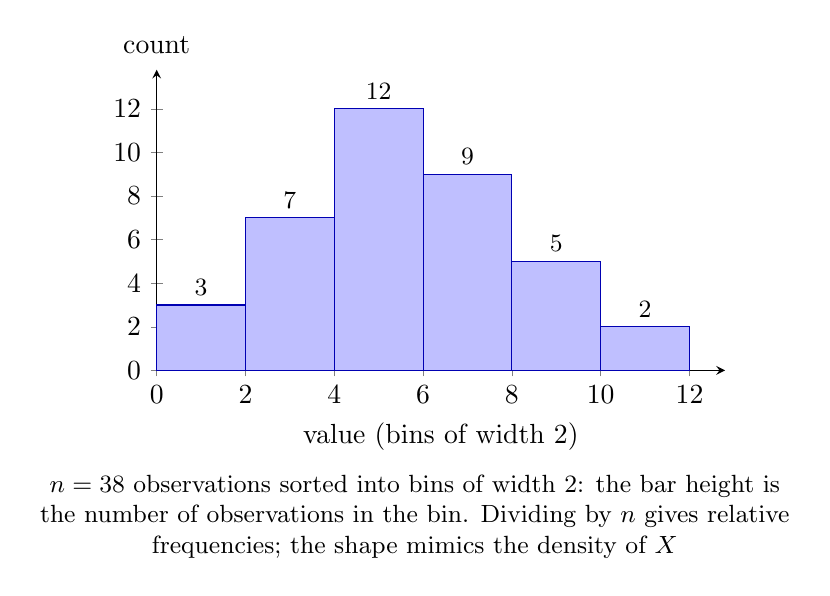
\begin{tikzpicture}
	\begin{axis}[
		axis lines=left, xmin=0, xmax=12.8, ymin=0, ymax=13.8,
		xtick={0,2,...,12}, ytick={0,2,...,12},
		xlabel={value (bins of width $2$)}, ylabel={count}, ylabel style={rotate=-90, anchor=south, at={(axis description cs:0,1.02)}},
		width=8.8cm, height=5.4cm, clip=false
		]
		\addplot[ybar, bar width=2, fill=blue!25, draw=blue!70!black] coordinates {(1,3) (3,7) (5,12) (7,9) (9,5) (11,2)};
		\node[font=\small, anchor=south] at (axis cs:1,3) {$3$};
		\node[font=\small, anchor=south] at (axis cs:3,7) {$7$};
		\node[font=\small, anchor=south] at (axis cs:5,12) {$12$};
		\node[font=\small, anchor=south] at (axis cs:7,9) {$9$};
		\node[font=\small, anchor=south] at (axis cs:9,5) {$5$};
		\node[font=\small, anchor=south] at (axis cs:11,2) {$2$};
	\end{axis}
	\node[anchor=north, font=\small, align=flush center, text width=9.6cm] at ([yshift=-2pt]current axis.outer south) {$n=38$ observations sorted into bins of width $2$: the bar height is the number of observations in the bin. Dividing by $n$ gives relative frequencies; the shape mimics the density of $X$};
\end{tikzpicture}
\end{document}
